\chapter{Software}
The Sensor Board hardware has two programmable CPUs and several configurable chips. The main ESP32 CPU (two low-power Xtensa 32-bit LX6 microprocessors) \cite{espressif:ESP-WROOM-32} is programmable via USB or Bluetooth or JTAG. The JTAG connector is not present on the Sensor Board. The second microcontroller is a part of BMF055 \cite{bosch:BMF055} multifunctional chip. It is Atmel SAMD20 \cite{atmel:SAMD20} with ARM Cortex-M0+ CPU programmable via SWD interface \cite{SWDinterface}.

\paragraph{Microcontrollers:}
\begin{enumerate}
	\item Espressif ESP-WROOM-32 \cite{espressif:ESP-WROOM-32}:
		\begin{itemize}
			\item dual core, 240 MHz, 448 kB ROM, 520 kB SRAM, 4 MB SPI flash memory
			\item Designated for main program handling all communication and interaction with user or other devices.
		\end{itemize}
	\item Atmel SAMD20 \cite{atmel:samd20}:
		\begin{itemize}
			\item ARM Cortex-M0+ CPU, 48 MHz, 32 kB SRAM, 256 kB flash memory
			\item Designated for processing inertial data and computing sensor fusion, can be used for example as an emulator of other sensors or as a simple flight controller.
		\end{itemize}
\end{enumerate}

\begin{figure}
	\centering
	\label{fig:SWmodules}
	\caption{Schema of the available modules inside the SensorBoard hardware}
	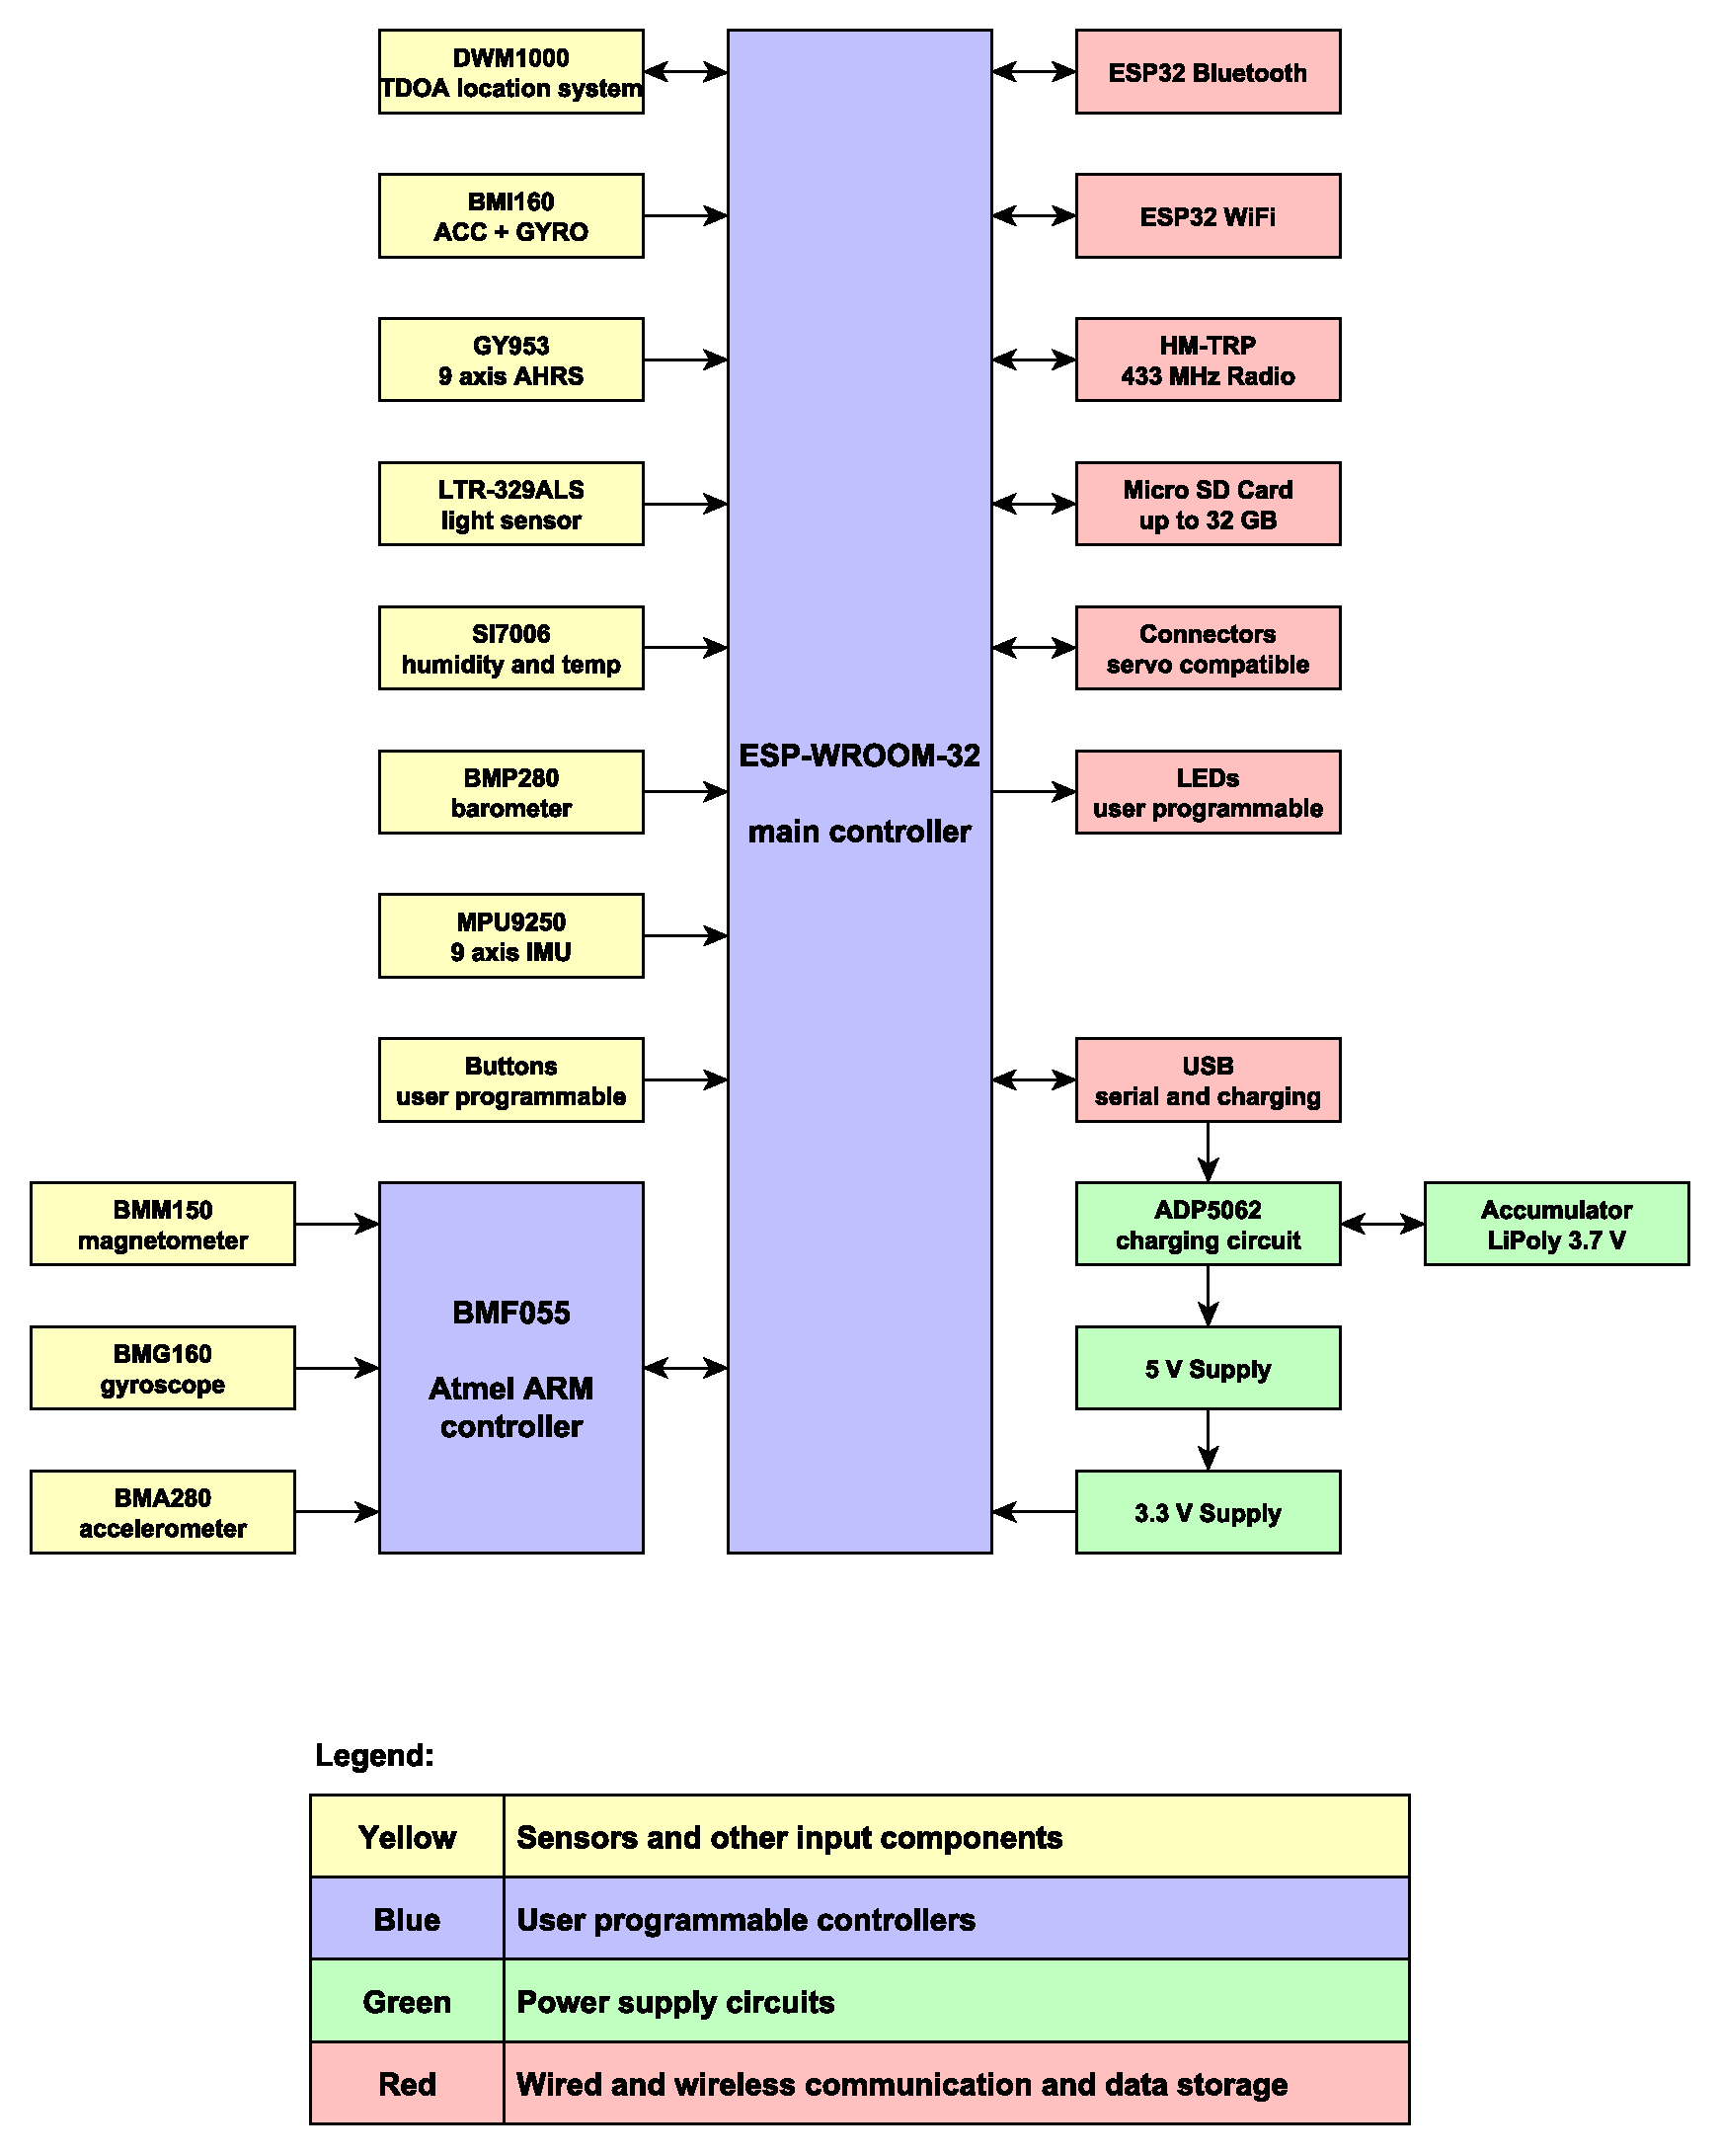
\includegraphics[width=16cm]{img/SensorBoardSchema.pdf}
\end{figure}

\section{Programming the Board}
Each processor on the Sensor Board has to be programmed separately via its interface. Only ESP32 \cite{espressif:ESP-WROOM-32} (main processor) can be programmed over the air via Bluetooth. This feature is disabled by default. The pinout an other information about the SensorBoard and BMF055 board are described in appendix \ref{hardwareDocumentation}.

\subsection{Programming ESP32}
There are several ways how to program and use the ESP32 \cite{espressif:ESP-WROOM-32} controller. The official framework is Espressif IoT Development Framework (ESP-IDF) \cite{espressif:ESP-IDF} and supports all the chip functionality. The ESP-IDF framework is POSIX compatible.

The chip can be programmed using Arduino compatible framework \cite{espressif:ArduinoCore} which creates an easy way for prototyping and learning, but does not offer all the functionality of the chip. The Arduino framework uses the ESP-IDF framework, so we can create "hybrid" programs that use both frameworks.

The last mentioned programming method is scripting in Python. We can upload the MicroPython \cite{MicroPython} firmware directly to the ESP32 controller. The Python libraries, scripts and other data are stored on the SD card. The MicroPython firmware supports most of the hardware functionality, but there are still some restrictions.

There are some other ways how to create a program for this hardware, but many of them use one of the mentioned frameworks. For example we can create a program in Simulink and then export it for the ESP32 controller. \cite{ArduinoSimulink}

\subsubsection{ESP-IDF Framework}
The ESP-IDF framework is almost POSIX compatible. \cite{ESP32posix} It supports many POSIX compatible functions, but it still doesn't support all of them. It means that we can compile many POSIX compatible programs for ESP32, but not all of them.

We can follow the official ESP32 programming guide \cite{ESP32programmingGuide} to setup the environment and program the board. The user can do everything from terminal (command line). The figure \ref{ESP32menuconfig} shows a configuration tool used for setup the program before the first compilation and upload to the ESP32 microcontroller.

\begin{figure}
	\centering
	\label{ESP32menuconfig}
	\caption{Configuration of the ESP-IDF program in terminal before the first compilation}
	\includegraphics[width=16cm]{img/ESP32menuconfig.png}
\end{figure}

If we prefer some GUI for development of our software we have several options. I will mention two of them:
\begin{enumerate}
	\item \textbf{Eclipse IDE} can be setup using the guide in ESP-IDF Programming Guide \cite{ESP32eclipse}. In my opinion, the compilation of our programs is very slow when we use this option. The figure \ref{ESP32eclipse} shows the SensorBoard project opened in Eclipse IDE.
	\item \textbf{PlatformIO IDE} is an open source ecosystem for IoT development. \cite{PlatformIO} There is integrated ESP-IDF and Arduino framework for ESP32 microcontrollers. This option was more familiar for me with much faster compilation process. I have used the PlatformIO ecosystem inside Atom \cite{AtomEditor} advanced text editor. The figure \ref{ESP32atom} shows the SensorBoard project opened in Atom editor with PlatformIO plugin.
\end{enumerate}

\begin{figure}
	\centering
	\label{ESP32eclipse}
	\caption{The SensorBoard project opened in Eclipse IDE}
	\includegraphics[width=16cm]{img/ESP32eclipse.png}
\end{figure}

\begin{figure}
	\centering
	\label{ESP32atom}
	\caption{The SensorBoard project opened in Atom text editor with PlatformIO plugin}
	\includegraphics[width=16cm]{img/ESP32atom.png}
\end{figure}

\subsubsection{Arduino Compatibility}
The Arduino compatible framework for ESP32 \cite{espressif:ArduinoCore} is dependent on ESP-IDF framework \cite{espressif:ESP-IDF}. It means that we can use both -- the ESP-IDF functions and the Arduino functions -- in our programs. The Arduino framework is primarily targeted for begineers and for fast prototyping. I don't recommend to use this framework for advanced applications, because it doesn't cover the whole ESP32 functionality. We can develop our Arduino compatible programs in Arduino IDE, but we can use the PlatformIO ecosystem, too. It means that we can use the same environment like in the figure \ref{ESP32atom}. All libraries are donwloaded and installed automatically inside the PlatformIO. We have to set only a \texttt{platformio.ini} file in the root directory of our project. We can add a line \texttt{framework = arduino} for Arduino compatible programs and a line \texttt{framework = espidf} for programs using the ESP-IDF framework.

\subsubsection{MicroPython Compatibility}
The builded MicroPython binary for ESP32 can be directly downloaded from MicroPython website. \cite{MicroPython} We can directly flash this binary to our ESP32 controller (to the SensorBoard) and then diretcly run our Python scripts. Of course, it is possible to download the MicroPython source code from the same website. The MicroPython allows to control the SensorBoard via Python serial terminal, so we can send separate command via this serial terminal or run the whole Python scripts stored as files in the SD card. The SD card slot is a part of the SensorBoard. One of the Python scripts on the SD card can be configured to be executed automatically after powering on the SensorBoard. The running Python serial terminal on the SensorBoard is shown in figure \ref{ESP32PythonLorris}.

\begin{figure}
	\centering
	\label{ESP32PythonLorris}
	\caption{The running Python serial terminal on the SensorBoard}
	\includegraphics[width=16cm]{img/PythonESP.png}
\end{figure}

\subsection{Programming BMF055}
The BMF055 \cite{bosch:BMF055} is a custom programmable 9-axis motion sensor. It is a single chip triaxial accelerometer, dynamic gyroscope, magnetometer and ARM controller. The BMF055 chip is mounted on a separate board which can be optionally mounted to the SensorBoard or it can be used independently. The figure \ref{BMF055photo} shows the separate BMF055 board and the same board mounted to the SensorBoard.

\begin{figure}
	\centering
	\label{BMF055photo}
	\caption{The separate BMF055 board on the left and the same board mounted to the Sensor board on the right}
	\begin{minipage}[c]{.45\textwidth}
		\includegraphics[width=7cm]{img/BMF055.jpg}
	\end{minipage}
	\vrule{}
	\begin{minipage}[c]{.45\textwidth}
		\includegraphics[width=7cm]{img/HWassembledNoCoin.jpg}
	\end{minipage}
\end{figure}

The BMF055 board has several usages, because it contains a user programmable controller. It can be used for example as a simple UAV controller or autopilot. The project BMF055-flight-controller \cite{BMF055flightController} implemented this single chip autopilot solution for multicopters.

The Atmel SAM D20 controler \cite{atmel:samd20} can be programmed in Atmel Studio \cite{AtmelStudio} and the program can be flashed to the chip via SWD interface \cite{SWDinterface}. We have to use Atmel ICE programmer \cite{AtmelICE} or similar hardware. For details about configuration and programming of the BMF055 chip we can follow the BMF055 datasheet \cite{bosch:BMF055} or the Atmel SAM D20 datasheet \cite{atmel:samd20}. The pinout of the BMF055 board and other hardware details are described in Appendix \ref{BMF055pinNumbering}. The figure \ref{BMF055AtmelStudio} shows an opened BMF055 project in Atmel Studio 7.

\begin{figure}
	\centering
	\label{BMF055AtmelStudio}
	\caption{An opened BMF055 project in Atmel Studio 7}
	\includegraphics[width=16cm]{img/BMF055AtmelStudio.png}
\end{figure}

\section{Application Programming Interface}
The programming interface for the SensorBoard can be split to several categories. There is a native support from the manufacturer of the microcontrollers. This API is written for any electronic device with the targeted microcontroller and this API is mentioned in section \ref{GeneralAPI}.

I have implemented a new library for easier working with the sensors present on the SensorBoard.

\subsection{SensorBoard API}
//todo

\subsection{General API for the controllers}
\label{GeneralAPI}
Both controllers used on the SensorBoard have an API defined and implemented by the manufacturer.

\paragraph{Atmel SAM D21:} \cite{AtmelSAMd20API}
\begin{multicols}{2}
\begin{itemize}
	\setlength\itemsep{1pt}
	\item AC -- Analog Comparator (Callback APIs)
	\item ADC -- Analog-to-Digital Converter (Polled APIs)
	\item T30TSE75X Temperature Sensor
	\item AT45DBX DataFlash
	\item AVR2025 -- IEEE 802.15.4 MAC Stack v3.1.1
	\item AVR2025 -- TAL
	\item AVR2025 -- TFA
	\item AVR2025-MAC Serial Interface Module
	\item AVR2130 -- LW MESH v1.2.1
	\item BOD -- Brown Out Detector
	\item CRC-32 calculation
	\item CRC32 -- 32-bit cyclic redundancy check
	\item DAC -- Digital-to-Analog Converter (Callback APIs)
	\item Debug Print (FreeRTOS)
	\item Delay routines
	\item EEPROM Emulator Service
	\item Ethernet Physical Transceiver (ksz8851snl)
	\item EVSYS -- Event System with interupt hooks support
	\item EXTINT -- External Interrupt (Polled APIs)
	\item FatFS file system
	\item Generic board support
	\item GFX Monochrome -- Menu System
	\item GFX Monochrome -- Monochrome Graphic Library
	\item GFX Monochrome -- Spinner/Spin control widget
	\item GFX Monochrome -- System Font
	\item Interrupt management -- SAM implementation
	\item IOPORT -- General purpose I/O service
	\item Memory Control Access Interface
	\item NVM -- Non-Volatile Memory
	\item PAC -- Peripheral Access Controller
	\item Performance Analyzer Application
	\item PORT -- GPIO Pin Control
	\item QTouch Library for SAMD20/D21
	\item RTC -- Real Time Counter in Calendar Mode (Callback APIs)
	\item RTC -- Real Time Counter in Count Mode (Callback APIs)
	\item SAM D20/D21 implementation of AT25DFx SerialFlash with vectored master SPI
	\item SD/MMC stack on SPI interface
	\item SERCOM I2C -- Slave Mode I2C (Polled APIs)
	\item SERCOM SPI -- Serial Peripheral Interface (Callback APIs)
	\item SERCOM SPI -- Serial Peripheral Interface (Master Mode, Vectored I/O)
	\item SERCOM USART -- Serial Communications (Polled APIs)
	\item Serial I/O -- Host using UART
	\item Serial I/O -- NCP Using UART
	\item Sleep manager -- SAMD implementation
	\item Smart Card
	\item SSD1306 OLED controller
	\item Standard serial I/O (stdio)
	\item SYSTEM -- Clock Management for SAMD20
	\item SYSTEM -- I/O Pin Multiplexer
	\item TC -- Timer Counter (Callback APIs)
	\item Unit test framework -- SAM0 implementation
	\item USART -- Serial interface -- SAM implementation for devices with only USART
	\item WDT -- Watchdog Timer (Polled APIs)
\end{itemize}
\end{multicols}

\paragraph{Espressif ESP-WROOM-32:} \cite{ESP32API}
\begin{multicols}{2}
\begin{itemize}
	\item Wi-Fi
	\begin{itemize}
		\setlength\itemsep{1pt}
		\item Wi-Fi
		\item Smart Config
		\item ESPNOW
	\end{itemize}
	\item Mesh
	\begin{itemize}
		\setlength\itemsep{1pt}
		\item ESP Mesh
	\end{itemize}
	\item Bluetooth
	\begin{itemize}
		\setlength\itemsep{1pt}
		\item Bluetooth Controller \&\& VHCI
		\item Bluetooth Common
		\item Bluetooth LE
		\item Bluetooth Classic
	\end{itemize}
	\item Ethernet
	\begin{itemize}
		\setlength\itemsep{1pt}
		\item Ethernet
	\end{itemize}
	\item Peripherals
	\begin{itemize}
		\setlength\itemsep{1pt}
		\item ADC
		\item DAC
		\item GPIO (including RTC low power I/O)
		\item I2C
		\item I2S
		\item LED Control
		\item MCPWM
		\item Pulse Counter
		\item Remote Control
		\item SDMMC Host
		\item SD SPI Host
		\item Sigma-delta Modulation
		\item SPI Master
		\item SPI Slave
		\item Timer
		\item Touch Sensor
		\item UART
	\end{itemize}
	\item Protocols
	\begin{itemize}
		\setlength\itemsep{1pt}
		\item mDNS
		\item ESP-TLS
	\end{itemize}
	\item Storage
	\begin{itemize}
		\setlength\itemsep{1pt}
		\item SPI Flash and Partition APIs
		\item SD/SDIO/MMC Driver
		\item Non-Volatile Storage
		\item Virtual Filesystem
		\item FAT Filesystem
		\item Wear Levelling
		\item SPIFFS Filesystem
	\end{itemize}
	\item System
	\begin{itemize}
		\setlength\itemsep{1pt}
		\item FreeRTOS
		\item FreeRTOS Hooks
		\item Heap Memory Allocation
		\item Heap Memory Debugging
		\item Interrupt Allocation
		\item Watchdogs
		\item Inter-Processor Call
		\item High Resolution Timer
		\item Logging
		\item Application Level Tracing
		\item Power Management
		\item Sleep Modes
		\item Base MAC address
		\item Over The Air Updates (OTA)
		\item ESP pthread
	\end{itemize}
	\item Configuration Options
	\begin{itemize}
		\setlength\itemsep{1pt}
		\item Kconfig
	\end{itemize}
\end{itemize}
\end{multicols}







\subsubsection{Software Tools}
- SW vlastnosti jako POSIX kompatibilita, FreeRTOS atd.



\section{Usage Examples}
- priklady naprogramovani - logovani jen ESP, sensorfusion na BMF, navigace na ESP a vypocty na BMF atd., flight controller na BMF + na ESP user commands, indoor location service

\section{Data Logging Firmware}
//todo: samostatna kapitola?
- SW pro analyzu namerenych dat
- jak funguje sbirani dat, synchronizace jednotlivych casti atd.

//todo: citovat vetsi verzi ESP WROOM 32 a vypsat vyhody